\chapter{Standortplanung auf Netzwerken} % (fold)
\label{cha:standortplanung_auf_netzwerken}

  \label{sec:standortplanung_auf_netzwerken}

  \section{Graphentheorie} % (fold)
  \label{sec:graphentheorie}

    \par \textbf{Gewichteter ungerichteter Graph $G = (V, E)$}
    \begin{itemize}
        \item $V = {v_1, \dots, v_n}$: eine nichtleeren Menge von Knoten  
        \item $E = {e_1, \dots, e_m}$: Menge von Kanten
      \end{itemize}  

    \par \textbf{Ungerichtetes Netzwerk $N = (G, l)$}
    \begin{itemize}
      \item $G = (V, E)$: ein gewichteten ungerichteten Graphen
      \item $l:E \rightarrow \mathbb{R}_+: l_{ij} := l(e), e= [v_i, v_j]$: Kantenbewertung (Länge der Kante)
    \end{itemize}

    \par \textbf{Wege}

    $P(v_i, v_j) = (v_i = v_{i_1}, e_{j_1},v_{i_2}, e_{j_2}, \dots, v_{i_{t - 1}}, e_{j_{t-1}}, v_{i_t} = v_j)$

    \par Kurz: $P(v_i, v_j) = (v_1, v_2, \dots, v_{i_{t-1}}, v_j)$

    \par Gilt $v_i = v_j \Rightarrow$ Zyklus $Z$ 

    \par Länge eines Weges: 
    \[
      l(p):= \sum_{s = 1, \dots, t-1}l(e_{j_s})
    \]

    \par \textbf{Zusamenhang}

    \par Ein Graph heißt zusammenhängend, falls je zwei Knoten durch einen Weg miteinander verbunden sind.

    \par \textbf{Baum}
    \par Ein Baum $T = (V,E)$ ist ein zyklusfreier, zusammenhaängender Graph, d. h. jedes Paar Knoten ist durch genau einen Weg miteinander verbunden.
    \par Die Endknoten eines Baums nennt man Blatt-Knoten oder kurz Blätter. Ein Blatt ist mit genau einem anderen Knoten des Baums adjazent.

    \par \textbf{Teilgraph}
    \par $G' = (V', E')$ ist ein Teilgraph von $G= (V,E)$, falls $V' \subseteq V$ und $E' \subset E$ und für alle Kanten $e = [v_i, v_j] \in E'$ gilt, dass $v_i, v_j \in V'$
    \par $G'$ heißt \textbf{spanneder Teilgraph}, falls $V' = V$

    \par \textbf{Distanz zwischen zwei Knoten}
    \par Die Distanz $d(v_i, v_j)$ zwischen zwei Knoten $v_i$ und $v_j \in V$ entspricht der Länge eines kürzesten Weges $P'(v_i, v_j)$ zwischen $v_i$ und $v_j$

    \[
    d(v_i, v_j) := l(P'(v_i, v)j) := \text{min}\{l(P(v_i,v_j))|P(v_i, v_j) ein Weg von v_i nach v_j\}
    \]
    
    \begin{itemize}
      \item symmetrisch
      \item nicht-negativ
      \item $d(v_i, v_i) = 0$ für alle $v_i \in V$
    \end{itemize}

    \par \textbf{Punkte des Netzwerks}
    \par Ein Punkt $x$ auf einer Kante $e = [v_i, v_j]$ ist definiert als Paar $x = ([v_i, v_j], t), 0 \leq t \leq 1$ mit $d(x, v_i) = t \cdot l(e)$ und $d(x, v_j) = (1-t)\cdot l(e)$

    \begin{itemize}
      \item $([v_i, v_j], 0) = v_i$
      \item $([v_i, v_j], 1) = v_j$
    \end{itemize}

    \par $P(G)$: die Menge aller Punkte $\Rightarrow V \subseteq P(G)$

    \par \textbf{Distanz zwischen Punkt und Knoten}
    \par Sei $x = ([v_i, v_j], t) \in P(G)$ und $v_k \in V$
    \[
      \text{Distanz zwischen } x \text{ und } v_k := \text{Länge eines kürzesten Weges von } x \text{ nach } v_k
    \]

    \par \textbf{Bottleneck-Punkte}

    \par Ein Punkt $x$ auf Kante $e = [v_i, v_j]$ heißt \textbf{Bottleneck-Punkt (BNP) des Knoten $v_k$ }, falls
    \[
      d(x, v_i) + d(v_i, v_k) = d(x, v_j) + d(v_j, v_k)
    \]
    d.h.die kürzestenWege von $x$ nach $v_k$ über $v_i$ bzw. $v_j$ haben identische Länge.

    \par Bezeichnung: $BN_{ij}^k$ Bottleneck-Punkt des Knotens $v_k$ auf der Kante $[v_i, v_j]$

    \par Für einen Bottleneck-Punkt $BN_{ij}^k$ des Knotens $v_k$ auf der Kante $[v_i, v_j]$ gilt

    \begin{equation*}
      \begin{aligned}
        & d(x, v_i) + d(v_i, v_k) = d(x, v_j) + d(v_j, v_k) \\
        & \Leftrightarrow tl_{ij} + d_{ik} = (1-t)l_{ij} + d_{jk} \\
        & \Leftrightarrow 2tl_{ij} = l_{ij} + d_{ik} - d_{ik} \\
        & \Leftrightarrow t = \frac{l_{ij} + d_{jk} - d_{ik}}{2l_{ij}} =: t_{ij}^k    
        \end{aligned}
    \end{equation*}
      


    \par Bestimmung aller Bottleneck-Punkte einer Kante $[v_i, v_j]$:
    Berechne $t_{ij}^k$ für alle Knoten $v_k \in V$. Gilt $0 < t_{ij}^k < 1$, so liegt ein BNP vor, sonst nicht.

  % section graphentheorie (end)

  \section{1-Medianprobleme} % (secfold)
  \label{sec:1_medianprobleme}

    \par Platziere eine neue Einrichtung so auf dem Netzwerk, dass die Summe der gewichteten Entfernungen von dem neuen Standort zu den Knoten minimal wird.

    \par \textbf{Zielfunktion}

    \[
      f(x) := \sum_{i = 1}^{n}w_id(x, v_i), x \in P(G)
    \]

    \begin{itemize}
      \item Knotenbeschränktes: $\underset{v \in V}{\text{min}}f(v)$
      \item Absolutes: $\underset{x \in P(G)}{\text{min}}f(v)$
    \end{itemize}

    \par \textbf{Dominanzkriterium}
    \par Gilt für einen Knoten $v_k$ mit zugehörigem Gewicht $w_k$, dass
    \[
      w_k \geq \frac{1}{2}\sum_{i = 1, \dots, n}w_i
    \]

    \subsection{1-Medianprobleme auf allgemeinen Graphen} % (fold)
    \label{sub:1_medianprobleme_auf_allgemeinen_graphen}

      \subsubsection{Knotenbeschränktes 1-Medianproblem} % (fold)
      \label{ssub:knotenbeschränktes_1_medianproblem}

        \begin{enumerate}
          \item Berechne die gewichtete Distanzmatrix
                $$
                  diag(w_1, \dots, w_n) \cdot D = 
                  \begin{pmatrix}
                    w_1d(v_1, v_1) &  \cdots & w_1d(v_n, v_1) \\
                    \vdots  & \ddots & \vdots  \\
                    w_1d(v_1, v_n) & \cdots & w_1d(v_n, v_n)
                 \end{pmatrix}
                $$
                (Zeile $i$ enthält die gewichteten Entfernungen von $v_i$ zu allen anderen Knoten $v_j: w_id(v_j, v_i)$
          \item Die Spalte mit der \textbf{kleinsten Spaltensumme} liefert einen Median.
        \end{enumerate}

        \begin{exmp}
          
        \end{exmp}

        \begin{figure}[H]
          \centering
          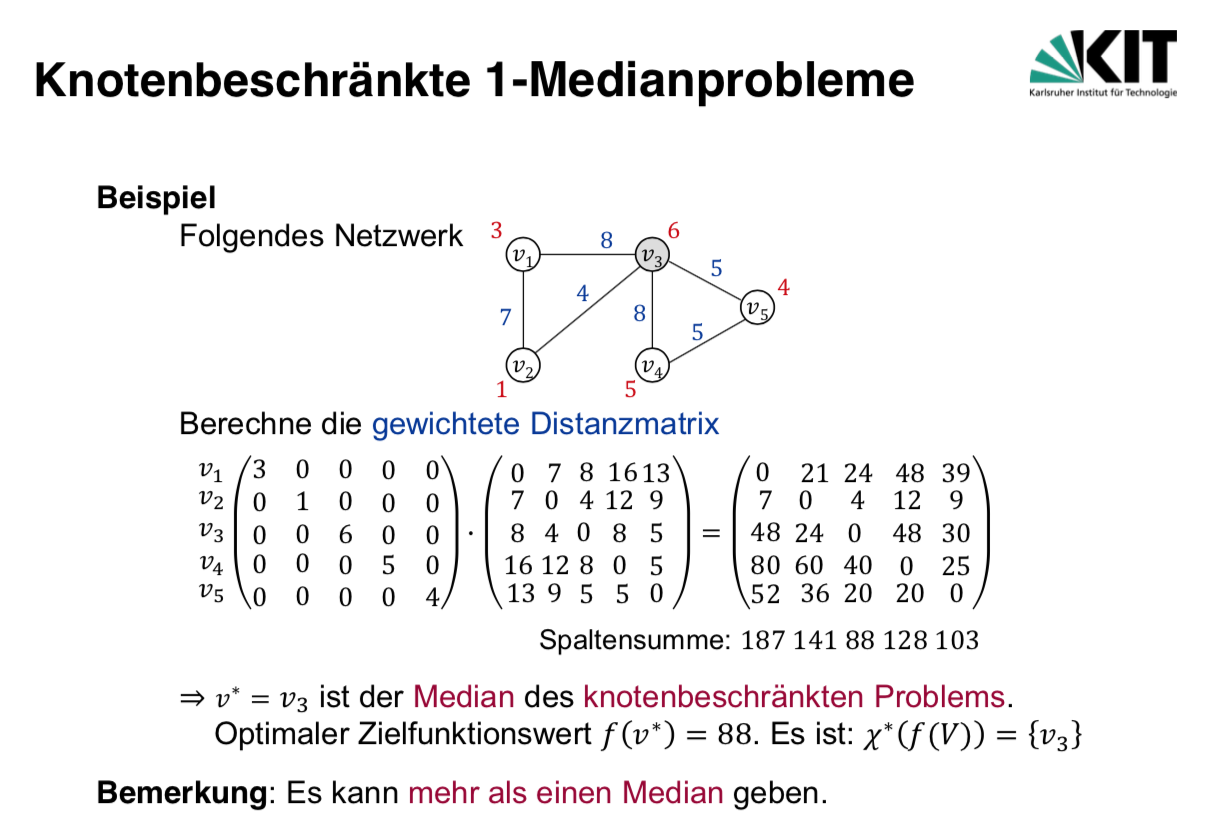
\includegraphics[width=0.95\textwidth]{Images/Knotenbeschraenktes_1_median_Problem_Bsp.png}
          \caption{Knotenbeschränktes 1-Medianproblem Bsp}
          \label{fig:Knotenbeschraenktes_1_median_Problem_Bsp}
        \end{figure}

      % subsubsection knotenbeschränktes_1_medianproblem (end)

      \subsubsection{Absolutes 1-Medianproblem} % (fold)
      \label{ssub:absolutes_1_medianproblem}

        \par \textbf{Zielfunktion}
        $$
        f(x):= \sum_{i = 1}^{n}w_id(x, v_i), x = (e,t), 0 \leq t \leq 1
        $$

        \par \textbf{Hakimi-Knotendominanzkriterium}
        Man findet unter den Knoten bereits einen absoluten Median:
        \[
          \mathcal{X}^*(f(G)) \cap V \neq \varnothing
        \]

        \par \textbf{Lösungsverfahren}: Verwende das Verfahren für das knotenbeschränkte Problem zur Bestimmung eines absoluten Medians.

        \begin{itemize}
          \item Ist die Summe aller Gewichte ungerade, d. h. $\sum_{i = 1, \dots, n}w_i$, so gilt: $\mathcal{X}^*(f(G)) \subseteq V$
          \item Sind zwei adjazente Knoten optimal und ein beliebiger Punkt auf der Kante dazwischen ebenfalls, so ist die gesamte Kante optimal.
        \end{itemize}

        \begin{exmp}
          
        \end{exmp}

        \begin{figure}[H]
          \centering
          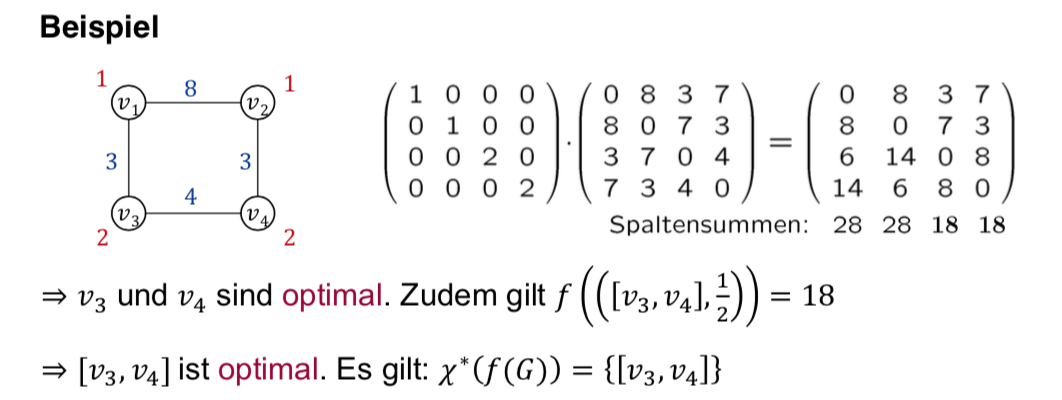
\includegraphics[width=0.95\textwidth]{Images/Absolut_1_Medianproblem.png}
          \caption{Absolut 1 Medianproblem Bsp}
          \label{fig:Absolut_1_Medianproblem-Bsp}
        \end{figure}
       
      % subsubsection absolutes_1_medianproblem (end)
    
    % subsection 1_medianprobleme_auf_allgemeinen_graphen (end)

    \subsection{1-Medianprobleme auf Bäume} % (fold)
    \label{sub:1_medianprobleme_auf_b_ume}

      \begin{algorithm}[H]
        \begin{algorithmic}
          \caption{Einklapp Verfahren von Goldmann}
          \State 1. Berechne $W = w(V)$
          \State 2. Gilt $T = \{v_i\}$, so $v^* := v_i \Rightarrow$ Stopp!\\ 
          Sonst wähle eine Blatt-Kante $e = [v_i, v_j]$ von $T$ mit Blatt $v_i$\\ 
          Falls $w_i \geq \frac{W}{2}$, so $v^* := v_i \rightarrow$ Stopp! (Gilt $w_i = \frac{W}{2}$, so ist die komplette Kante $[v_i, v_j]$ optimal.)
          \State 3. Setze $w_j:= w_j + w_i$ und lösche $v_i$ und $[v_i, v_j]$ aus T.\\ 
          Gehe zu Schritt 2.
          % \EndProcedure
        \end{algorithmic}
      % \textbf{Output:} 
      \end{algorithm}

      \begin{exmp}
        
      \end{exmp}

      \begin{figure}[H]
        \centering
        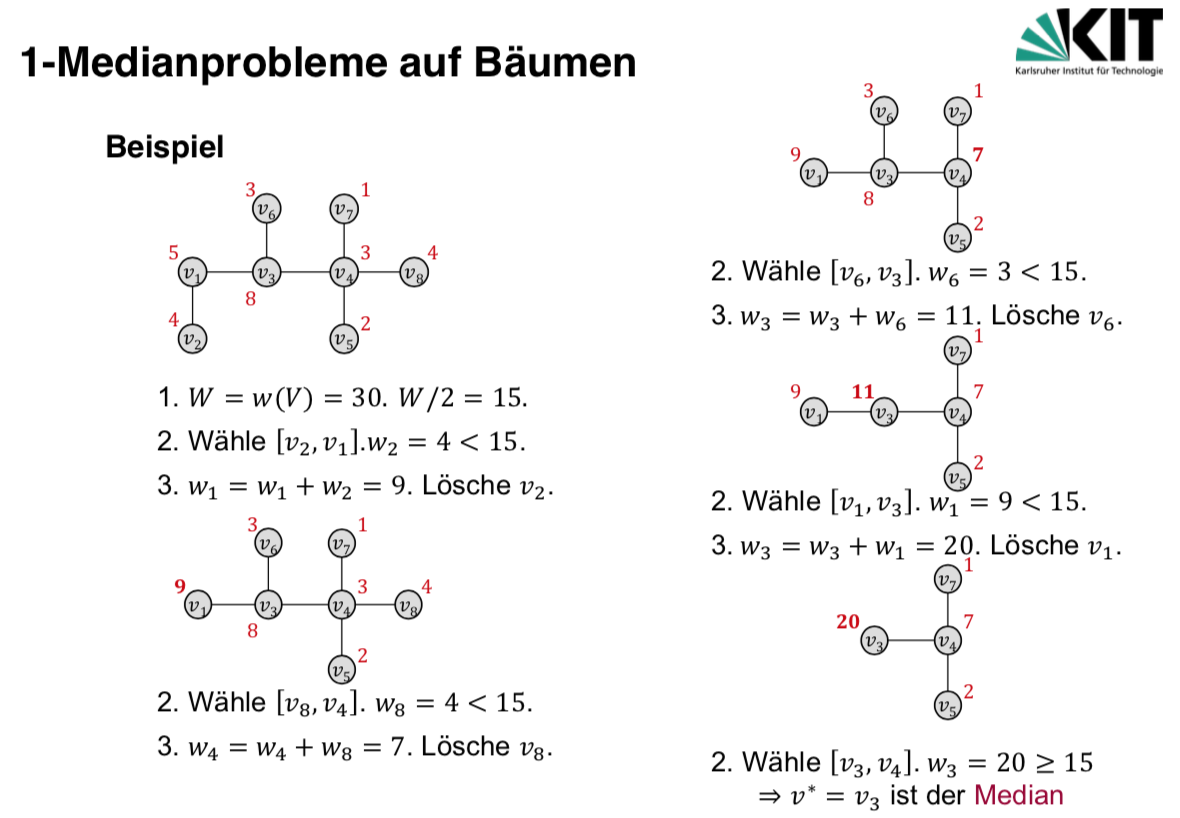
\includegraphics[width=0.95\textwidth]{Images/1_Medianproblem_auf_Baeume_Bsp.png}
        \caption{1 Medianproblem auf Bäume}
        \label{fig:1_Medianproblem_auf_Baeume_Bsp}
      \end{figure}
    % subsection 1_medianprobleme_auf_b_ume (end)
  
  % section 1_medianprobleme (end)

  \section{1-Centerprobleme} % (fold)
  \label{sec:1_centerprobleme}

    \par Platziere eine neue Einrichtung so auf dem Netzwerk, dass die maximale gewichtete Entfernung von dem neuen Standort zu den Knoten minimal wird.

    \par \textbf{Zielfunktion}

    \[
      g(x) := \underset{i= 1, \dots, n}{\text{max}}w_i\cdot d(x, v_i), x \in P(G)
    \]
  
    \subsection{1-Centerprobleme auf allgemeinen Graphen} % (fold)
    \label{sub:1_centerprobleme_auf_allgemeinen_graphen}

      \par \textbf{Zielfunktion}: $\underset{v \in V}{\text{min}}g(v)$


      \par \textbf{Lösungsverfahren}
      \begin{enumerate}
        \item Berechne die gewichtete Distanzmatrix
              $$
                diag(w_1, \dots, w_n) \cdot D = 
                \begin{pmatrix}
                  w_1d(v_1, v_1) &  \cdots & w_1d(v_n, v_1) \\
                  \vdots  & \ddots & \vdots  \\
                  w_1d(v_1, v_n) & \cdots & w_1d(v_n, v_n)
               \end{pmatrix}
              $$
              
        \item Bestimme für jede Spalte den \textbf{maximalen Eintrag} in der Spalte. Die Spalte mit dem \textbf{kleinsten maximalen Eintrag} liefert einen Center.
      \end{enumerate}

      \begin{exmp}
        
      \end{exmp}

      \begin{figure}[H]
        \centering
        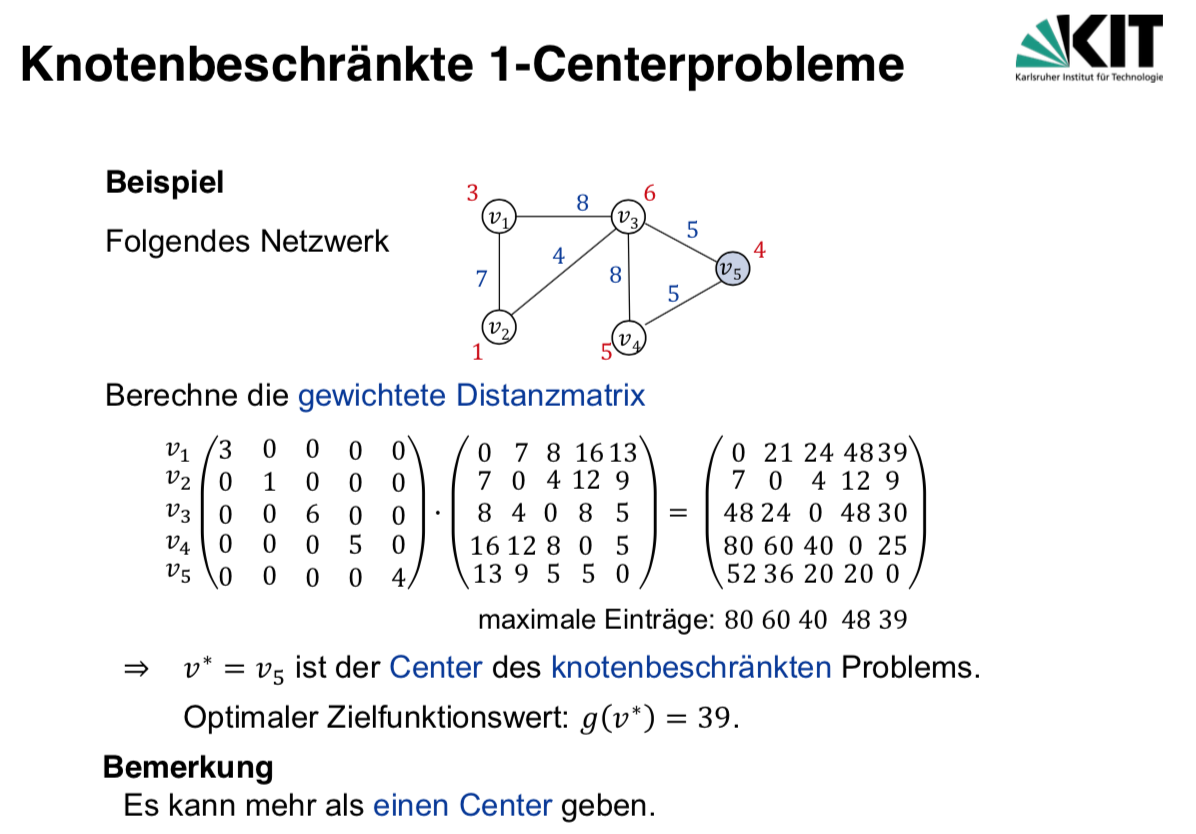
\includegraphics[width=0.95\textwidth]{Images/Knotenbeschraenktes_1_Centerproblem_Bsp.png}
        \caption{Knotenbeschraenktes 1-Centerproblem Bsp}
        \label{fig:Knotenbeschraenktes_1_Centerproblem_Bsp}
      \end{figure}

    % subsection 1_centerprobleme_auf_allgemeinen_graphen (end)

    \subsection{1-Centerprobleme auf Bäume} % (fold)
    \label{sub:1_centerprobleme_auf_b_ume}
      
      \par Sowohl das absolute als auch das knotenbeschränkte Problem auf Bäumen mit nicht-identischen Knotengewichten wird mit den Verfahren der vorherigen Abschnitte für allgemeine Graphen gelöst.
      
      \par Für ungewichtete Probleme gibt es effizientere Verfahren.

      \subsubsection{Das ungewichtete 1-Centerproblem} % (fold)
      \label{ssub:das_ungewichtete_1_centerproblem}

      \par \textbf{Zielfunktion}
      \[
        g(x) := \underset{i=1,\dots, n}{\text{max}}d(x, v_i), x \in P(T)
      \]

      Der absolute, ungewichtete Center eines Baums ist der Mittelpunkt eines längsten Weges zwischen zwei Knoten im Baum.

      \begin{algorithm}[H]
        \begin{algorithmic}[1]
          \caption{Verfahren für absolute 1-Centerprobleme auf Bäume}
          \State Wähle einen beliebigen Punkt $x \in P(T), T = (V, E)$
          \State Bestimme den \textbf{am weitesten} von $x$ entfernt liegenden Knoten $v$ in $T$.
          \[d(v,x):= \underset{i=1, \dots, n}{\text{max}}d(v_i, x)\]
          \State Bestimme den \textbf{am weitesten} von $v$ entfernt liegenden Knoten $v'$ in $T$
          \[d(v', v) := \underset{i = 1, \dots, n}{\text{max}}d(v_i, v)\]
          \State $x* = \text{Mittelpunkt von } P(v, v'): d(x^8, v) = d(x^*, v') = \frac{1}{2}d(v, v') = g(x^*)$
          % \EndProcedure
        \end{algorithmic}
      % \textbf{Output:} 
      \end{algorithm}

      \begin{exmp}
        
      \end{exmp}

      \begin{figure}[H]
        \centering
        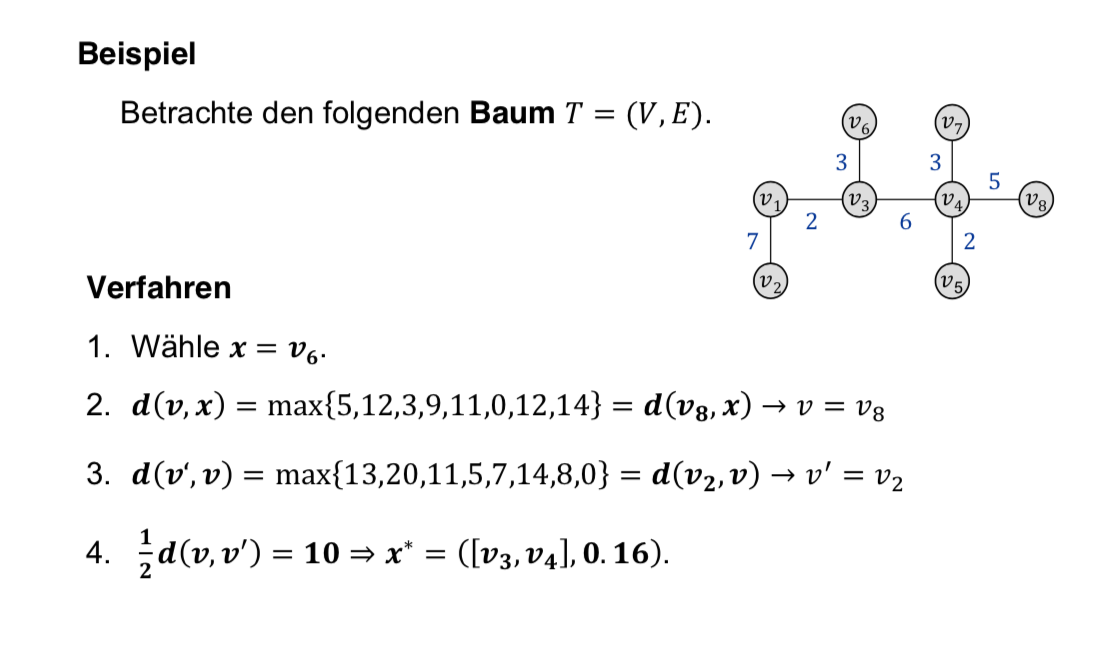
\includegraphics[width=0.95\textwidth]{Images/Absolut_1_Centerproblem_auf_ungewichtete_Baeume_Bsp.png}
        \caption{Absolute 1-Centerproblem auf ungewichtete Baeume Bsp}
        \label{fig:Absolut_1_Centerproblem_auf_ungewichtete_Baeume_Bsp}
      \end{figure}

      \par \textbf{Das knotenbeschränkte Problem}

      \par Sei $x^* = ([v_i, v_j], t)$ ein absoluter Center auf der Kante $e = [v_i, v_j]$
      \par Dann ist einer der Endknoten der Kante $[v_i, v_j]$ ein Center:
      \[g(x^*) := \text{min}\{g(v_i), g(v_j)\}\]

      \begin{exmp}
        
      \end{exmp}

      \begin{figure}[H]
        \centering
        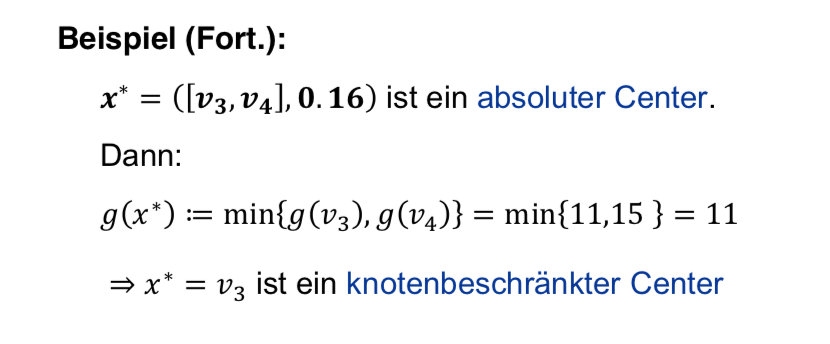
\includegraphics[width=0.95\textwidth]{Images/Knotenbeschr_1_Centerproblem_auf_ungewichtete_Baeume_Bsp.png}
        \caption{Knotenbeschränktes 1-Centerproblem auf ungewichtete Baeume Bsp}
        \label{fig:Knotenbeschr_1_Centerproblem_auf_ungewichtete_Baeume_Bsp}
      \end{figure}
      % subsubsection das_ungewichtete_1_centerproblem (end)
    % subsection 1_centerprobleme_auf_b_ume (end)

  % section 1_centerprobleme (end)

  \section{Mehrstandortprobleme} % (fold)
  \label{sec:mehrstandortprobleme}
  
  % section mehrstandortprobleme (end)
% chapter standortplanung_auf_netzwerken (end)




    
